\documentclass[final]{beamer}
\mode<presentation>{\usetheme{I6pd2}}
\usepackage[english]{babel}
\usepackage[latin1]{inputenc}
\usepackage{subfig}
\usepackage{amsmath,amsthm, amssymb, latexsym}
%\usepackage{times}\usefonttheme{professionalfonts}  % obsolete
\usefonttheme[onlymath]{serif}
\boldmath
\usepackage[orientation=landscape,size=a0,scale=1.4,grid]{beamerposter}
\usepackage{natbib}
% change list indention level
%\setdefaultleftmargin{3em}{}{}{}{}{}

\usepackage{snapshot} % will write a .dep file with all dependencies, allows for easy bundling
\usepackage{epstopdf}

\listfiles

%%%%%%%%%%%%%%%%%%%%%%%%%%%%%%%%%%%%%%%%%%%%%%%%%%%%%%%%%%%%%%%%%%%%%%%%%%%%%%%%%%%%%%
\graphicspath{{figures/}}
 
\title{\huge REU Fish Tracking Project}
%\subtitle{Presentation Subtitle} % (optional)

%% author and in []: shortauthor
\author{Joseph Anderson, Brian Lewis, Colin O'Byrne}
% - Use the \inst{?} command only if the authors have different
%   affiliation.
\institute[University of New Orleans] % (optional, but mostly needed)
{
%  \inst{1}%
 Training and Research in Advanced Computing Knowledge, University of New Orleans, Louisianna
%  \and
%  \inst{2}%
%  Department of Theoretical Philosophy\\
%  University of Elsewhere
}
% - Use the \inst command only if there are several affiliations.
% - Keep it simple, no one is interested in your street address.

\date[12 July 2011]{12 July 2011}
%%%%%%%%%%%%%%%%%%%%%%%%%%%%%%%%%%%%%%%%%%%%%%%%%%%%%%%%%%%%%%%%%%%%%%%%%%%%%%%%%%%%%%
\newlength{\columnheight}
\setlength{\columnheight}{65cm}

%%%%%%%%%%%%%%%%%%%%%%%%%%%%%%%%%%%%%%%%%%%%%%%%%%%%%%%%%%%%%%%%%%%%%%%%%%%%%%%%%%%%%%
\begin{document}
\begin{frame}
  \begin{columns}
    % ---------------------------------------------------------%
    % Set up a column 
    \begin{column}{.33\textwidth}
      \begin{beamercolorbox}[center,wd=\textwidth]{postercolumn}
        \begin{minipage}[T]{.95\textwidth} % tweaks the width, makes a new \textwidth
          \parbox[t][\columnheight]{\textwidth}{ % must be some better way to set the the height, width and textwidth simultaneously
            % Since all columns are the same length, it is all nice and tidy.  You have to get the height empirically
            % ---------------------------------------------------------%
            % fill each column with content            
            \begin{block}{Introduction}
              The goal is to extract and classify fish data from natural underwater video data.  To do this, we use automatic thresholding methods to segment the image and the segmented fish are interpreted by either a system of neural networks or feature extraction algorithms.  We study the performance of different threshold methods and the accuracy of various neural network structures.  WARP methods and Gabor filters are used as classification tools alongside the neural networks.
            \end{block}
            \vfill
            \begin{block}{Data Flow Diagram}
              \centering
              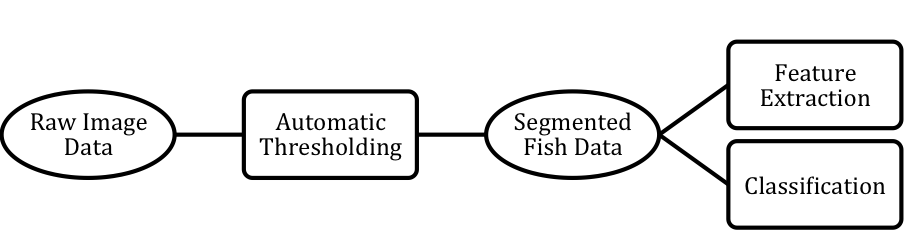
\includegraphics[width=.95\linewidth]{figures/process2}
            \end{block}
            \vfill
            \begin{block}{Sample Image Data}
              \centering
              \begin{figure}
                \centering
                \caption{An original image with the detected fish}
                \subfloat[An original fish image]{\label{fig:originalimage}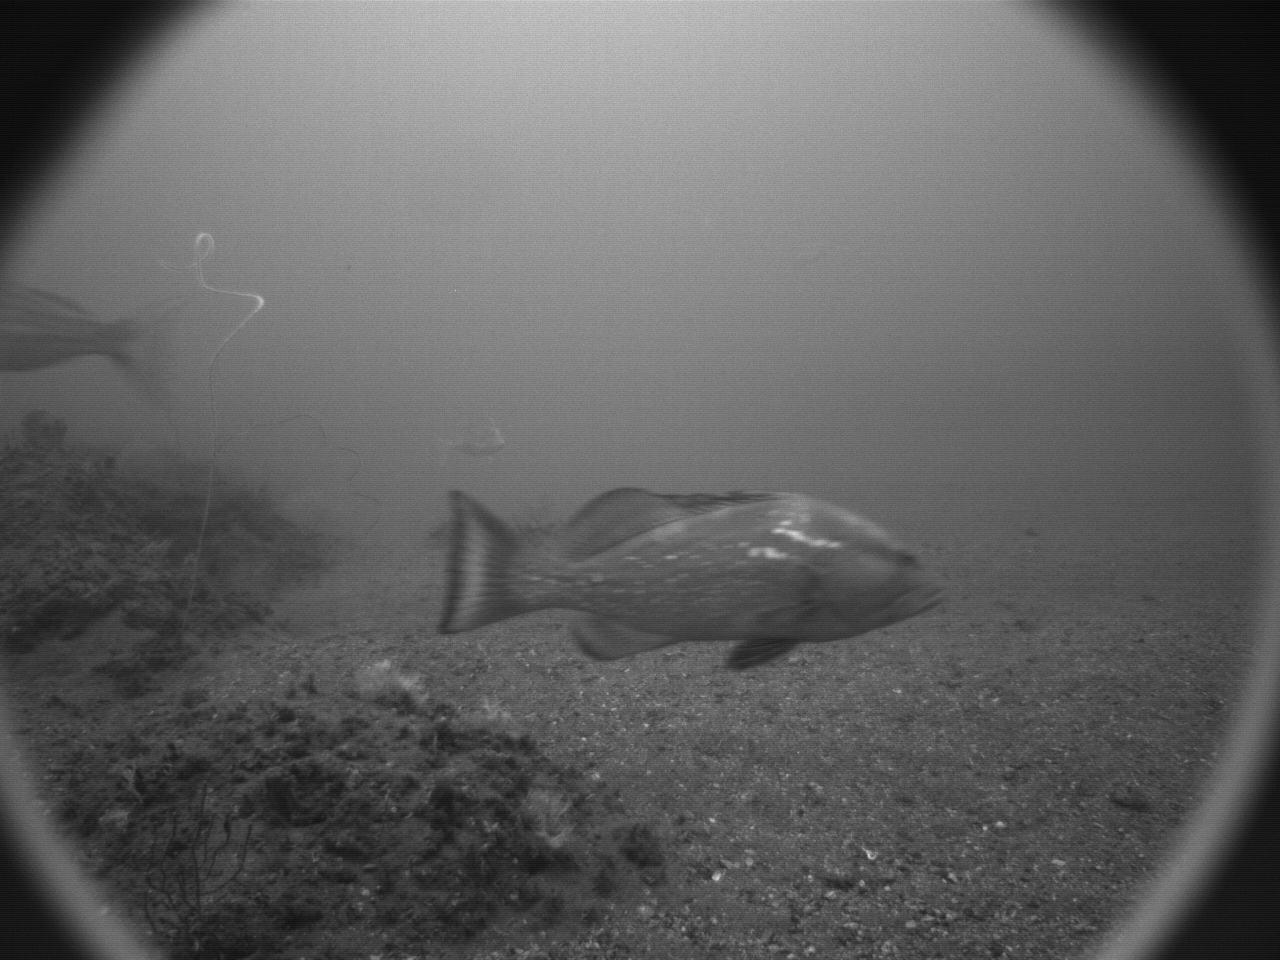
\includegraphics[scale=0.25]{figures/fishoriginal} } \quad
                \subfloat[Fish detected by Tao graph cut algorithm]{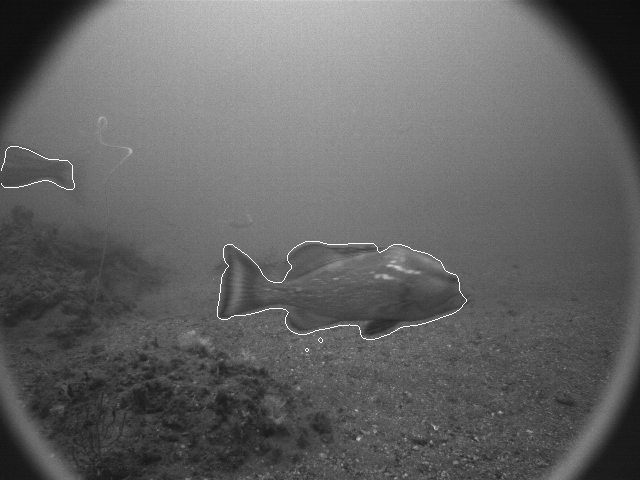
\includegraphics[scale=0.5]{figures/threshdemo2tao}}
              \end{figure}
            \end{block}
            \vfill
            \begin{block}{Thresholding Methods}
              \begin{itemize}
              	\item Histogram
			\begin{itemize}
				\item Otsu / Liao \emph{et al}. - maximizes class variance (Liao \emph{et al}. improve performance)
				\item Ramesh \emph{et al}. - minimize either sum of square error or sum of variance
			\end{itemize}
		\item Clustering
			\begin{itemize}
				\item Kittler and Illingworth - minimize a Gaussian-based criterion
			\end{itemize}
		\item Entropy
			\begin{itemize}
				\item Guo - maximize standard shannon entropy
				\item Ajlan - maximize cross-entropy of gamma distribution
				\item Xiao - calculate Gaussian entropy of two-dimensional gray level spatial correlation histogram
			\end{itemize}
		\item Graph Cut
			\begin{itemize}
				\item Tao - minimize naturalized cut with optimized method
			\end{itemize}
              \end{itemize}
            \end{block}
          }
        \end{minipage}
      \end{beamercolorbox}
    \end{column}
    % ---------------------------------------------------------%
    % end the column

    % ---------------------------------------------------------%
    % Set up a column 
    \begin{column}{.33\textwidth}
      \begin{beamercolorbox}[center,wd=\textwidth]{postercolumn}
        \begin{minipage}[T]{.95\textwidth} % tweaks the width, makes a new \textwidth
          \parbox[t][\columnheight]{\textwidth}{ % must be some better way to set the the height, width and textwidth simultaneously
            % Since all columns are the same length, it is all nice and tidy.  You have to get the height empirically
            % ---------------------------------------------------------%
            % fill each column with content
            
            \begin{block}{WARP}
	      \begin{itemize}
              \item Makes use of Duscrete Fourier Transforms (DFT) for reduced dimensionality.
	      \item Modifies DFT coefficents to retain phase, magnitude, and starting point information.
	      \item Dynamic Time Warping (DTW) used to calculate distance, allows for deformities in image shape.
	      \item Sakoe-Chiba band is used to make DTW computations much quicker.
	      \end{itemize}
            \end{block}
            \vfill
            \begin{block}{WARP Results}
              \begin{itemize}
	      \item Euclidian Distance Comparison: 21.2\% recognition rate
              \item WARP Direct Image Comparison: 53.2\% recognition rate
              \item WARP Average Distance Compariosn: 86.4\% recogniton rate
              \end{itemize}              
            \end{block}
            \vfill
            \begin{block}{Gabor Filters for Different Fish Species}
              \centering
              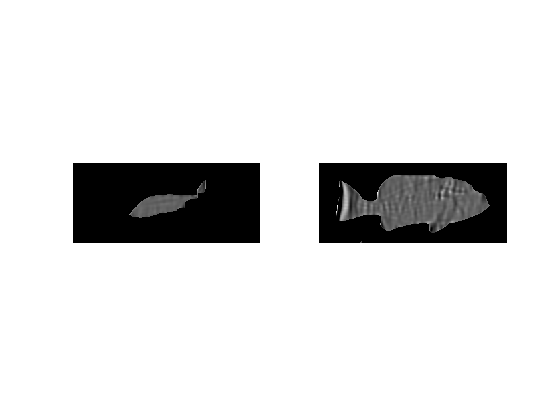
\includegraphics[width=.95\linewidth,scale = .6,clip=true,trim=0 100 0 100]{figures/Gabor}
            \end{block}
            \vfill
            \begin{block}{Gabor Filters}
              \begin{itemize}
              \item Identify E. morio based on stripe on tail
              \item Ratio of horizontal and and vertical Gabor filters highlights stripe
              \item Presence of stripe indicates E. morio, process had 
              \end{itemize}              
            \end{block}
            \vfill
            \begin{block}{Segmentation of \ref{fig:originalimage}}
             \begin{figure}
               \centering
               \caption{FIsh segments with and without edge thinning}
               \subfloat[Kitter's method without thinning]{ 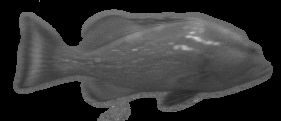
\includegraphics[scale=1.1]{figures/subdemokittler} }
               \subfloat[Tao's method without thinning]{ 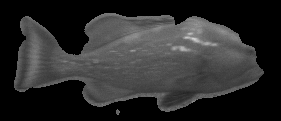
\includegraphics[scale=1.1]{figures/subdemotao} }
               \subfloat[Xiao's method without thinning]{ 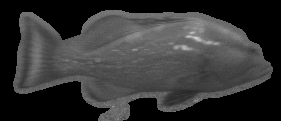
\includegraphics[scale=1.1]{figures/subdemoxiao} }
               
               \subfloat[Kitter's method with thinning]{ 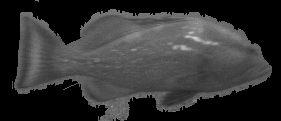
\includegraphics[scale=1.1]{figures/subdemokittlerthin} }
               \subfloat[Tao's method with thinning]{ 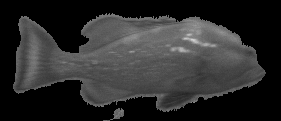
\includegraphics[scale=1.1]{figures/subdemotaothin} }
               \subfloat[Xiao's method with thinning]{ 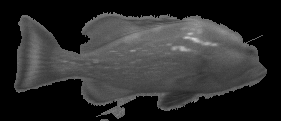
\includegraphics[scale=1.1]{figures/subdemoxiaothin} }
             \end{figure}
             
            \end{block}
          }
        \end{minipage}
      \end{beamercolorbox}
    \end{column}
    % ---------------------------------------------------------%
    % end the column

    % ---------------------------------------------------------%
    % Set up a column 
    \begin{column}{.33\textwidth}
      \begin{beamercolorbox}[center,wd=\textwidth]{postercolumn}
        \begin{minipage}[T]{.95\textwidth} % tweaks the width, makes a new \textwidth
          \parbox[t][\columnheight]{\textwidth}{ % must be some better way to set the the height, width and textwidth simultaneously
            % Since all columns are the same length, it is all nice and tidy.  You have to get the height empirically
            % ---------------------------------------------------------%
            % fill each column with content
            \begin{block}{Deep Belief Network}
                \begin{figure}[htbp]
                   \centering
                   \subfloat[RBM Architecture]{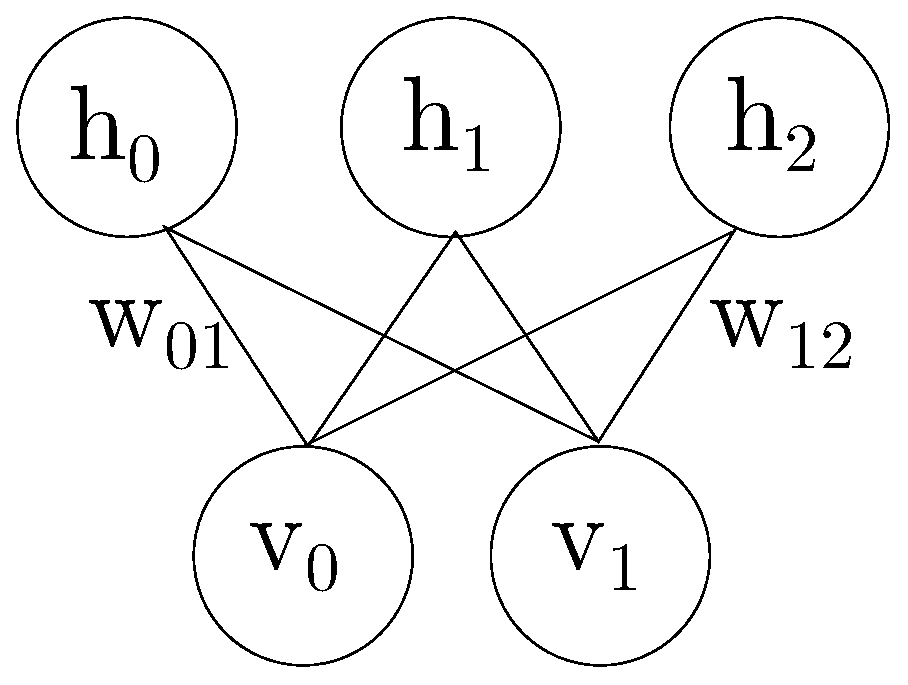
\includegraphics[height=5\baselineskip]{rbmarch}} % requires the graphicx package
                   \quad
                   \subfloat[DBN Architecture]{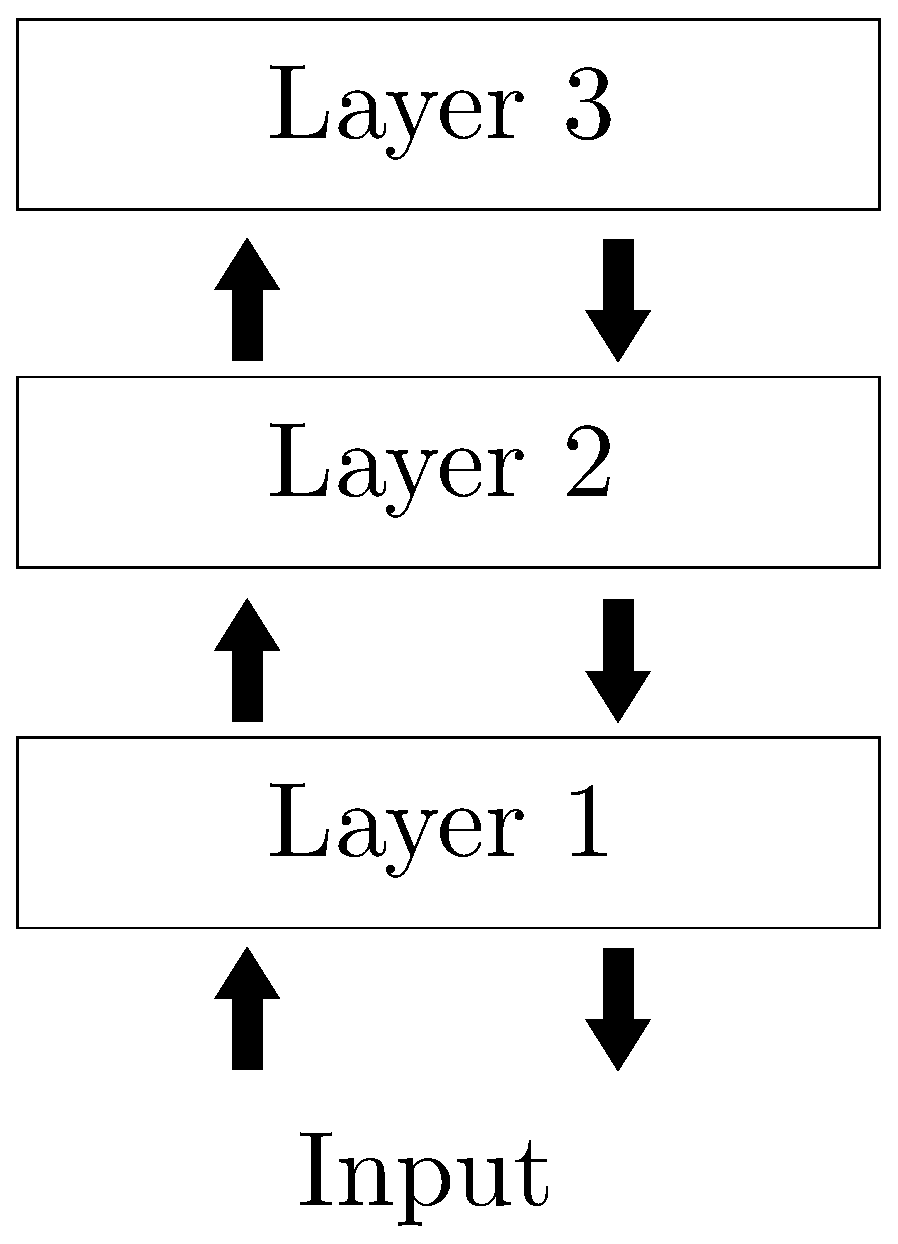
\includegraphics[height=5\baselineskip]{dbnarch}}
                   \label{fig:}
                \end{figure}
              \begin{itemize}
                  \item Learns a representation of input data
                  \item Might be able to reduce input noise and recover missing
                  data (due to obstructions or segmentation errors)
                  \item Each layer is a Restricted Boltzmann Machines
                  \item Can be efficiently trained by a greedy layer-by-layer
                  algorithm
              \end{itemize}              
            \end{block}
            \vfill
            \begin{block}{Convolutional Neural Network}
            \begin{figure}[htbp]
               \centering
               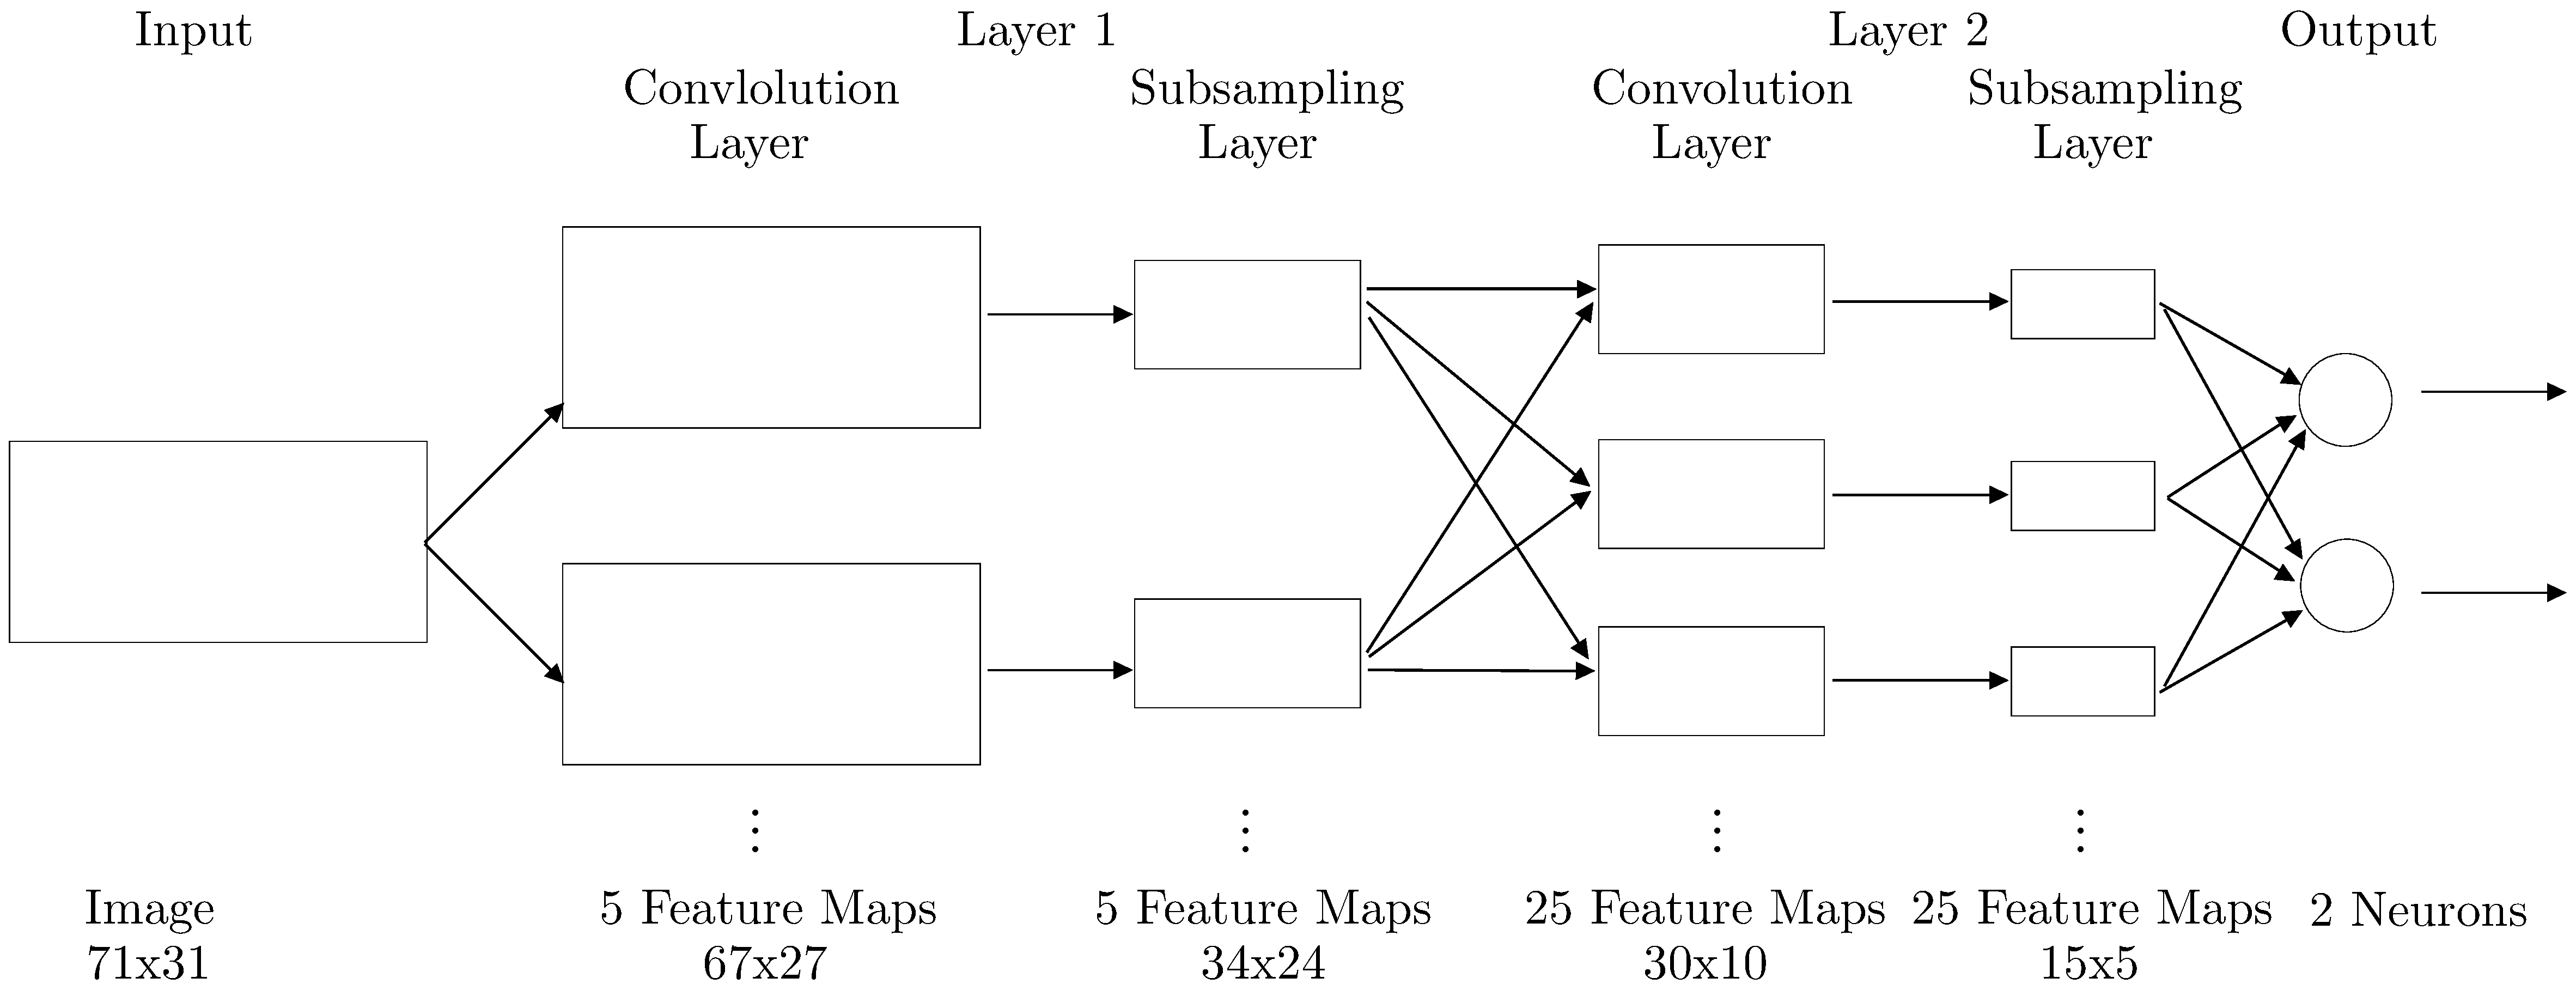
\includegraphics[height=5\baselineskip]{cnnarch} % requires the graphicx package
               \caption{CNN Architecture}
            \end{figure}
            \begin{itemize}
                \item Powerful architecture for image classification
                \item Preserves spatial information when extracting features
                \item High connectivity
                \item Efficient weight sharing
            \end{itemize}
            \end{block}
            \vfill
            \begin{block}{Classification Results}
              DBN
              \begin{itemize}
                \item Poor performance
                \item Model gets stuck at the local mimimum of an average of all
                inputs
                \item Different parameters and longer training might improve
                results
              \end{itemize}
             \bigskip
             CNN
             \begin{itemize}
                \item Good performance
                \item 88\% accuracy (74/84)
                \item Different architecture parameters may improve results
                further
             \end{itemize}
            \end{block}
            \vfill
%            \begin{block}{References}
%              \nocite{Xiao:2008vn}
%              \nocite{Tao:2008bh}
%	    \nocite{Kittler:1986zr}
%	    \nocite{Ila05}
%             \def\newblock{}\small
%	    \bibliographystyle{plain}
%  	    \bibliography{ImageProcessingBib}
%	    
%            \end{block}
          }
        \end{minipage}
      \end{beamercolorbox}
    \end{column}
    % ---------------------------------------------------------%
    % end the column


  \end{columns}
\end{frame}
\end{document}


%%%%%%%%%%%%%%%%%%%%%%%%%%%%%%%%%%%%%%%%%%%%%%%%%%%%%%%%%%%%%%%%%%%%%%%%%%%%%%%%%%%%%%%%%%%%%%%%%%%%
%%% Local Variables: 
%%% mode: latex
%%% TeX-PDF-mode: t
%%% End:
